% !TeX root=../main.tex
\chapter{ارزیابی و تحلیل نتایج}
%\thispagestyle{empty} 
\label{chap:results}
\section{مقدمه} 
در این فصل یک کاوش عمیق از مجموعه داده‌ها، مجموعه داده‌های آزمایشی، فراپارامترها، معیارهای ارزیابی و نتایج مورد استفاده در تحقیق ارائه شده است که با توصیف مجموعه داده‌های اولیه، از جمله ساختار، ویژگی‌ها و ارتباط آنها با حوزه شروع می‌گردد. 

این فصل به تشریح مجموعه داده‌های آزمایشی مورد استفاده برای اعتبارسنجی و مقایسه‌های مورد نیاز ادامه می‌دهد و به دنبال آن یک ارایه با جزییات از فراپارامترهای انتخاب‌شده برای بهینه‌سازی عملکرد مدل ارائه می‌شود. 

علاوه بر این، معیارهای ارزیابی مورد استفاده جهت تعیین کمیت اثربخشی مدل و تجزیه و تحلیل نتایج تجربی، از جمله آنالیز‌های حساسیت، برای ارزیابی استحکام رویکرد پیشنهادی تعریف شده‌است. این بحث جامع به اعتبار نتایج تحقیق کمک می‌کند.

\section{مجموعه داده‌های مورد استفاده}
در این قسمت دیتاست‌های مورد استفاده در این پژوهش توضیح‌داده شده است.


\subsection{مجموعه داده مووی‌لنز} 
همانطور که در بخش 
\ref{chap:dataset}
گفته شد، از دیتاست ۲۵ میلیونی مووی‌لنز استفاده شده است. این مجموعه داده‌های کاربران و فیلم ها، مانند رتبه‌بندی‌ها، ژانرها، و مُهرهای زمانی را ارائه می‌کند که پایه و اساس پروفایل‌سازی کاربر و وظایف پیشنهادی را تشکیل می‌دهند.

 مجموعه داده های موجود در مووی‌لنز به شرح زیر است:
\begin{enumerate}
\item
دیتاست فیلم‌ها:
ویژگی های این دیتاست به شرح زیر است
\begin{itemize}
\item
آیدی: یک شناسه منحصر به فرد برای هر فیلم. 
\item
عنوان: عنوان فیلم به همراه سال اکران آن. 
\item
ژانرها: فهرستی از ژانرهای مرتبط با فیلم.
\end{itemize}

\item
دیتاست امتیازها:
ویژگی های این دیتاست به شرح زیر است
\begin{itemize}
\item
آیدی کاربر: یک شناسه منحصر به فرد برای هر کاربر.
\item
آیدی فیلم: شناسه فیلم رتبه‌بندی‌شده توسط کاربر.
\item
امتیاز: امتیاز ارائه‌شده توسط کاربر، از 0.5 تا 5.0.
\item
مهر زمان: یک مهر زمانی یونیکس از زمانی که امتیاز داده‌شده‌ا‌ست.
\end{itemize}

\item
دیتاست تگ‌ها:
ویژگی‌های این دیتاست به شرح زیر است.
\begin{itemize}
\item
 آیدی کاربر: کاربری که تگ را اضافه کرده‌است.
\item
آیدی فیلم: شناسه فیلم تگ‌شده.
\item
 برچسب: تگ توصیفی اضافه‌شده توسط کاربر.
\item
مهر زمان: یک مهر زمانی یونیکس از زمانی که برچسب اضافه شده‌است.
\end{itemize}
\end{enumerate}

همچنین با استفاده از دیتاست‌های فوق، یک مجموعه داده تلفیقی از پیش پردازش شده MovieRatingTag ایجاد شده‌است.

 ویژگی‌های این مجموعه‌داده به صورت زیر است.
\begin{itemize}
\item
آیدی کاربر: شناسه کاربر.
\item
 آیدی فیلم: شناسه فیلم.
\item
 امتیاز: امتیاز کاربر برای فیلم.
\item
 عنوان: عنوان فیلم.
\item
 ژانرها: ژانرهای مرتبط.
\item
 برچسب: برچسب داده‌شده توسط کاربر، در صورت وجود.
\end{itemize}


\subsection{رویکردهای ایجاد مجموعه داده} 
با توجه به آن‌که جهت آموزش یک مدل زبانی بزرگ جهت ایجاد یک سیستم گفت‌وگو نیازمند دیتاستی با فرمت سوالات پرسیده و جواب‌های داده‌شده است، یک دیتاست به فرمت فوق ایجاد کردیم.

این مجموعه‌داده برگرفته از مووی‌لنز، مکالمه طبیعی را با ایجاد جفت پرسش-پاسخ شبیه سازی می‌کند. این مجموعه داده برای تکرارپذیری و استفاده سایرین در سایت هاگینگ فیس منتشر شده‌است. 

نحوه ایجاد این دیتاست به تفضیل در بخش 
\ref{chap:dataset}
آورده شده‌است.

ویژگی‌های مجموعه‌داده به شرح زیر است.
\begin{itemize}
\item
ورودی: اعلان ورودی که به سیستم گفتگو داده می‌شود.
\item
 خروجی: پاسخ مورد انتظار تولید‌شده توسط سیستم گفتگو.
\item
 عنوان فیلم: عنوان فیلم مربوط به دیالوگ.
\item
 سال: سال اکران فیلم.
\item
 ژانرها: ژانر(های) مرتبط با فیلم.
\item
امتیاز شباهت: امتیاز شباهت بین پاسخ‌های تولید‌شده و فیلم موجود در ورودی.
\end{itemize}	

یک نمونه از رکوردهای این دیتاست به فرمت زیر است.

 ورودی: من چند فیلم جنایی می خواهم که مانند«باشگاه مشت زنی (1999)» باشد. پیشنهاد شما چیست؟\\
 خروجی: پس از لذت بردن از «باشگاه مشت زنی (1999)»، فیلم‌های جنایی پنهان را کشف کنید. در اینجا چند پیشنهاد برای فیلم وجود دارد: Seven (1995)\\
 نام فیلم: باشگاه مشت زنی (1999)\\
 سال : 1995\\
 ژانر: اکشن | جنایی | درام | هیجان انگیز\\
 امتیاز شباهت: 
\num{0.93}\\


\section{مجموعه داده تست}
مجموعه‌داده مووی‌لنز برای استخراج پروفایل‌های کاربر، داده‌های آموزشی و داده‌های ارزیابی استفاده می‌شود.
نمایه‌های کاربران با تجزیه و تحلیل رتبه‌بندی کاربران، ژانرها و برچسب ها ساخته شده است.
\newline
داده‌های آموزشی شامل 80 درصد از دیتاست شخصی‌سازی‌شده کاربر و تعاملات وی است که برای تنظیم دقیق سیستم گفتگو استفاده می‌شود. با استفاده از این دیتاست، برای هرکاربر موجود در دیتاست یک مدل مجزا آموزش داده شده است که در مرحله ارزیابی مورد استفاده قرار گرفته‌ است.
\newline
داده‌های آموزشی شامل 20 درصد از دیتاست شخصی‌سازی‌شده کاربر و تعاملات وی برای ارزیابی استفاده شده است. ده نمونه تصادفی از هر کاربر برای آزمایش استفاده شد که با استفاده از مدل آموزش‌دیده‌شده خاص کاربر، مجموعه‌ای از جواب‌های شخصی‌سازی‌شده کاربر را ایجاد می‌کند که در نهایت پارامترهای ارزیابی بر روی این مجموعه داده‌ها اعمال خواهند شد.



\section{ابرپارامترها}
ابرپارامترها تنظیمات کلیدی در مدل‌های یادگیری ماشینی هستند که به طور قابل‌توجهی بر آموزش و عملکرد تأثیر می‌گذارند. برای این کار، ابرپارامترهای انتخاب‌شده بر روی تنظیم سریع و رفتار تولید مدل، و همچنین پیکربندی آموزش تمرکز دارند. در زیر به تفکیک هر یک از ابرپارامترها و تأثیر آن می‌پردازیم.
\subsection{فراپارامترهای تنظیم سریع و تولید پاسخ}

\begin{itemize}
\item
max-length

این مقدار حداکثر تعداد کلماتی را که مدل می‌تواند برای یک پاسخ ایجاد کند را تعیین می‌کند که ارزش 500 برای این مقدار در نظر گرفته شده‌است. 

 مقدار بالاتر، پاسخ‌های طولانی‌تر و دقیق را امکان‌پذیر می‌کند، اما زمان محاسبات و استفاده از حافظه را افزایش می‌دهد در حالی که مقادیر پایین‌تر می‌تواند طول پاسخ را محدود کند و به طور بالقوه پاسخ‌های معنی‌دار را کوتاه کند. مقدار انتخاب‌شده پرحرفی و کارایی محاسباتی را متعادل می‌کند.

\item
pad-token-id

شناسه پدتوکن، نشانه مورد استفاده‌ای است که فاصله‌های توالی به طول یکنواخت را مشخص می‌کند. 

اندازه ورودی ثابت و سازگاری با معماری مدل را تضمین می‌کند و از بروز خطا در طول آموزش یا استنتاج جلوگیری می‌کند. به همین دلیل مقدار tokenizer.eos-token-id برای این ابرپارامتر در نظر گرفته شده‌است.

\item
no-repeat-ngram-size

از تکرار هر اِن-گرام (توالی از n کلمه) در طول تولید توسط مدل جلوگیری می‌کند.

افزایش این مقدار تنوع در متن تولید‌شده را تشویق می‌کند، افزونگی را کاهش می‌دهد و منجر به پاسخ‌های طبیعی‌تر و متنوع‌تر می‌شود. برای این مقدار در آموزش مدل مقدار پنج انتخاب شده‌است.
\item
do-sample

نمونه‌ برداری از توزیع احتمال نشانه بعدی را به جای انتخاب همیشه نشانه با بیشترین احتمال (رمزگشایی حریصانه) فعال می‌کند.

 فعال‌کردن این مقدار در مدل تصادفی‌بودن را به پاسخ‌ها اضافه می‌کند و تنوع را افزایش می‌دهد.
 برای تولید خروجی‌های خلاقانه یا کمتر قطعی مفید است.
\item
top-k

 این ابرپارامتر در آموزش مدل تعداد توکن‌های بالقوه بعدی را به k محتمل‌ترین آن‌ها محدود می‌کند. مقدار در نظرگرفته‌شده برای این پارامتر 100 است.

افزایش مقدار این ابرپارامتر تصادفی‌بودن را به ادامه‌های قابل‌قبول‌تر محدود می‌کند. مقادیر بالاتر تنوع را افزایش می‌دهد اما می‌تواند منجر به پاسخ‌های منسجم کمتری شود.
\item
top-p

توکن‌هایی که احتمال تجمعی آن‌ها با تمرکز بر محتمل‌ترین نتایج تا p باشد را انتخاب می‌کند.

مقدار این ابرپارامتر تعادل بین رفتار قطعی و تصادفی را تضمین می‌کند. مقدار کمتر پاسخ‌های منسجم‌تری را در اولویت قرار می‌دهد.
\item
tempreture

این ابرپارامتر تصادفی‌بودن انتخاب نشانه را در طول تولید کنترل می‌کند.

مقادیر نزدیکتر به صفر مدل را قطعی تر می‌کند، در حالی که مقادیر بالاتر تغییرپذیری را ایجاد می‌کند. مقدار انتخاب شده
\num{0.8}
 است که خروجی‌های متنوع و نسبتاً منسجم را تضمین می‌کند.
\item
 target-device

سخت‌افزار مورد استفاده برای محاسبات را مشخص می‌کند. که با توجه به سیستم و سخت افزار  مقدار، "cuda" در صورت موجود‌بودن یا "cpu" در صورت عدم وجود حافظه گرافیکی مجزا انتخاب می‌شوند

 استفاده از جی‌پی‌یو به طور قابل توجهی سرعت آموزش و استنتاج را افزایش می‌دهد. همچنین مقدار سی‌پی‌یو سازگاری را در سیستم های بدون جی‌پی‌یو تضمین می‌کند.
\end{itemize}

\subsection{فراپارامترهای آموزشی}

\begin{itemize}
\item
learning-rate


این ابرپارامتر اندازه گام را برای به‌روزرسانی پارامترهای مدل در طول آموزش تعیین می‌کند.

 نرخ بالای یادگیری همگرایی را تسریع می‌کند، اما خطر فراتر رفتن از مقادیر بهینه را به‌همراه دارد که منجر به بی‌ثباتی می‌شود.  نرخ یادگیری تنظیم دقیق معمولا کمتر است (به عنوان مثال، 5e-5)، اما تنظیم سریع از مقادیر بالاتر برای تطبیق سریع جاسازی‌ها استفاده می‌کند. به همین دلیل مقدار 
\num{0.03}
 برای این ابرپارامتر در نظر گرفته شده است.
\item
 prompt-tuning-training-epoch

تعداد ایپاک%
\LTRfootnote{epoch}
‌ها‌ی کامل از مجموعه‌داده آموزشی را مشخص می‌کند.

دوره‌های بیشتر انطباق مدل را بهبود می‌بخشد، اما در صورت زیاده‌روی، خطر 
تطبیق بیش از حد%
\LTRfootnote{Overfitting}
 را دارد. مقدار انتخاب‌شده برای آموزش مدل پنچ ایپاک است عمق تمرین و کارایی زمان را متعادل می‌کند.

\item
 auto-find-batch-size

 با مقداردهی به این ابرپارامتر، مدل به صورت پویا بزرگترین اندازه دسته‌ای را که در حافظه جا می‌گیرد، تعیین می‌کند.

 راه‌اندازی آموزش را با جلوگیری از مشکلات سرریز حافظه ساده می‌کند و همچنین استفاده موثر از سخت‌افزار موجود را تضمین می‌کند.
\item
 no-cuda

اطمینان حاصل می‌کند که مدل در صورت وجود از منابع جی‌پی‌یو استفاده می کند.

 سرعت آموزش و توان عملیاتی مدل را بهبود می بخشد و همچنین سازگاری با هر دو سیستم جی‌پی‌یو و سی‌پی‌یو را تضمین می‌کند.
\end{itemize}

\subsection{تعامل ابرپارامترها}
\begin{itemize}
\item
 تعادل تصادفی و انسجام

 ترکیب top-k ،top-p و tempreture مستقیماً بر تنوع و طبیعی‌بودن پاسخ‌های تولید‌شده تأثیر می‌گذارد. ارزش‌های انتخاب شده به نفع خروجی‌های خلاقانه بدون قربانی کردن انسجام است.
\item
 ثبات آموزش مدل

 نرخ یادگیری بالاتر (3e-2) به‌روزرسانی‌های تعبیه‌شده را در طول تنظیم سریع تسریع می‌کند.
\item
 استفاده از منابع

 ویژگی‌هایی مانند auto-find-batch-size و پشتیبانی از جی‌پی‌یو تضمین می‌کند که فرآیند آموزش با منابع موجود سازگار می‌شود و کارایی را به حداکثر می‌رساند.
\end{itemize}

\section{معیارهای ارزیابی}
در این بخش، به معیارهای ازریابی مورد استفاده در ارزیابی سیستم گفتگو وظیفه‌گرا را بررسی می‌کنیم.

هدف از این معیارهای ارزیابی هم کیفیت پاسخ‌های تولید‌شده توسط مدل و هم میزان موفقیت سیستم گفتگو است. هر معیار بر جنبه‌های خاصی از سیستم، مانند موفقیت‌کار، رضایت کاربر، یا کیفیت پاسخ تمرکز می‌کند. در ادامه بحث مفصلی از معیارهای مربوطه، از جمله تعاریف، محاسبات و نقش آنها در ارزیابی ارائه شده است.

\subsection[معیار گیجی]{معیار گیجی\LTRfootnote{Perplexity}}

گیجی معیاری است برای اینکه یک مدل زبان احتمالی چقدر یک نمونه را پیش‌بینی می‌کند. این نشان دهنده عدم قطعیت مدل در تولید توکن بعدی در یک دنباله است.

\begin{equation}
\label{eq:perplexity}
P(W) = 2^{-\frac{1}{N} \sum_{i=1}^{N} \log_2 P(w_i | w_1, w_2, \ldots, w_{i-1})}
\end{equation}

در فرمول
\ref{eq:perplexity}
مقدار N  تعداد کل توکن ها در دنباله است.
همچنین P(wi) احتمالی که توسط مدل به توکن wi اختصاص داده شده است.


 گیجی کمتر نشان می دهد که مدل در پیش بینی نشانه بعدی بهتر است. در سیستم های گفتگو، گیجی روان بودن پاسخ و ارتباط پاسخ ها را ارزیابی می کند.

\subsection[معیار تمایز]{معیار تمایز\LTRfootnote{Distinct}}

مقاله%
\cite{li2015diversity}
به معیارهای ارزیابی تمایز برای ارزیابی تنوع پاسخ‌های تولید‌شده اشاره می‌کند. تمایز-n، تنوع متن تولیدشده را با محاسبه نسبت n-گرام منحصر‌به‌فرد به کل n-گرام در پاسخ‌ها اندازه گیری می‌کند.


معیار تمایز-1: تنوع یونیگرام‌ها (کلمات فردی) در متن تولیدشده را ارزیابی می‌کند.
\begin{LTR}
\begin{equation}
Distinct-1 = \frac{Number Of Unique Unigrams}{Total Number of unigrams}
\end{equation}
\end{LTR}

معیار تمایز-2: تنوع توالی دو کلمه‌ای‌ها در متن تولیدشده را ارزیابی می‌کند.
\begin{LTR}
\begin{equation}
Distinct-2 = \frac{Number Of Unique Bigrams}{Total Number Of Bigrams}
\end{equation}
\end{LTR}

 مقادیر بالاتر نشان‌دهنده پاسخ‌های متنوع‌تر و کمتر تکراری است که برای طبیعی‌بودن مکالمه بسیار مهم است.

\subsection[معیار میزان موفقیت]{معیار میزان موفقیت\LTRfootnote{Success Rate}}

میزان موفقیت یک معیار ارزیابی پرکاربرد برای سیستم‌های گفتگو، به ویژه در سیستم‌های گفتگوی وظیفه‌گرا است. این معیار به صورت کلی درصد اهداف موفق کاربر که توسط سیستم به‌دست‌آمده است را اندازه‌گیری می‌کند.

نرخ موفقیت به عنوان نسبت اهداف موفق کاربر به تعداد کل اهداف کاربر محاسبه می‌شود. هدف کاربر در صورتی موفق تلقی می‌شود که سیستم بتواند درخواست کاربر را برآورده کند یا کار را کامل کند%
\cite{sekulic2024reliable} .

در ارزیابی سیستم گفتگو فوق میزان موفقیت معادل آن است که هر چند وقت یکبار سیستم به یک نتیجه مثبت بر اساس بازخورد کاربر می‌رسد.

در این معیار محاسبه میزان موفقیت آسان است و آن‌ را به معیاری مناسب برای ارزیابی تبدیل می‌کند. همچنین درک روشنی از توانایی سیستم برای تحقق اهداف کاربر ارائه می‌دهد و میزان موفقیت امکان مقایسه سیستم‌های گفتگوی مختلف را فراهم می‌کند. 

فرمول محاسبه میزان موفقیت مطابق با 
\ref{eq:SuccessRate}
است.

\begin{LTR}
\begin{equation}
\label{eq:SuccessRate}
Success Rate = \frac{Number of 'LIKE' Feedbacks}{Total Feedbacks ('LIKE' + 'DISLIKE')}
\end{equation}
\end{LTR}

با استفاده از این معیار می‌توان توانایی سیستم در برآوردن انتظارات کاربر را ارزیابی کرد. همچنین بازخورد خنثی را برای تمرکز بر ترجیحات صریح کاربر در نظر گرفته نمی‌شود.


\subsection[معیار نرخ تکمیل]{معیار نرخ تکمیل\LTRfootnote{Completion Rate}}


نرخ تکمیل یک معیار ارزیابی است که برای ارزیابی عملکرد سیستم‌های گفتگو، به ویژه در سیستم‌های گفتگوی وظیفه‌گرا استفاده می‌شود. درصد مکالماتی که توسط سیستم با موفقیت انجام شده است را اندازه‌گیری می‌کند% 
\ref{sekulic2024reliable}
.

در واقع نرخ تکمیل کار، توانایی سیستم را برای انجام موفقیت‌آمیز یک کار در نوبت گفتگو اندازه‌گیری می‌کند. معیار تکمیل کار در سیستم گفتگو فوق، نشان‌دهنده موفقیت تکلیف‌محور، مانند ارائه توصیه‌های فیلم یا تکمیل هدف گفتگو است.
 
نرخ تکمیل به عنوان نسبت مکالماتی که معیارهای تکمیل را دارند به تعداد کل مکالمات آغاز شده محاسبه می‌شود.

معیارهای تکمیل به شرح زیر خواهد بود:
\begin{enumerate}
\item
پایان معتبر پیام تولید‌شده: 

متن تولید‌شده با علائم نگارشی معتبر (نشان دهنده پاسخ کامل) به پایان می‌‌رسد.
\item
توصیه فیلم: 

پاسخ حاوی توصیه حداقل یک فیلم است. بعد از دریافت گزاره تولیدشده توسط مدل ، فیلم‌های موجود در آن گزاره از آن استخراج  می‌گردد. این معیار خالی بودن یا نبودن این لیست از فیلم‌های پیشنهادی را بررسی می‌کند.
\end{enumerate}

فرمول محاسبه نرخ تکمیل مطابق با فرمول 
\ref{eq:CompletionRate}
است.

\begin{LTR}
\begin{equation}
\label{eq:CompletionRate}
Completion Rate = \frac{Number of Completed Tasks}{Total Number of Tasks}
\end{equation}
\end{LTR}



این معیار درکی واضح از تکمیل کار را ارائه می‌دهد.نرخ تکمیل نشانه واضحی از توانایی سیستم برای تکمیل مکالمات با موفقیت ارائه می‌دهد.
همچنین با در نظرگرفتن هر دو معیار، میزان تکمیل موفقیت جزئی را در نظر می‌گیرد، مانند مکالماتی که پایان معتبری دارند اما توصیه فیلم ندارند.

\subsection[معیار امتیاز تعامل کاربر]{معیار امتیاز تعامل کاربر\LTRfootnote{User engagement score metric}}

امتیاز تعامل کاربر سطح تعامل کاربران با سیستم را اندازه‌گیری می‌کند. این معیار با توجه به نشست‌های کاربر و بازخوردهایی که به سیستم داده است محاسبه می‌شود
\cite{es2023ragas}
.

برای هر کاربر به ازای هر نشست جدیدی که ایجاد می‌کند، تعداد جواب‌های تولیدی مدل که بازخورد مثبت گرفته‌اند را به تعداد کل پیام‌های ردو‌بدل‌شده مدل تقسیم می‌کند.

\begin{flushright}
\begin{equation}
UES = \left( \frac{Total Interactions in the Session}{Number Of 'LIKE' Feedbacks} \right) \times 10
\end{equation}
\end{flushright}

امتیاز تعامل کاربر بالاتر سیستم جذاب‌تری را پیشنهاد می‌کند.

\subsection[مطابقت تنوع نمایه]{مطابقت تنوع نمایه\LTRfootnote{Profile Diversity Match}}

مطابقت تنوع نمایه تنوع ژانرهای تحت پوشش توصیه‌های سیستم را در مقایسه با ترجیحات کاربر اندازه‌گیری می‌کند. این معیار در واقع ارزیابی می‌کند که سیستم تا چه حد از وسعت علایق کاربر به درستی در جواب‌های تولیدی خود استفاده کرده است.
\begin{equation}
PDM = \frac{Number Of Unique Recommended Genres}{Number Of Unique User-Preferred Genres}
\label{eq:PDM}
\end{equation}
   

 در فرمول 
\ref{eq:PDM}
ژانرهای توصیه‌شده منحصر به فرد برای کاربر در واقع  ژانرهای متمایز در توصیه‌های سیستم گفتگو در طول دوره ارزیابی هستند. همچنین ژانرهای منحصربه‌فرد ترجیحی کاربر، ژانرهای متمایز در نمایه کاربر هستند که در ابتدای ایجاد پروفایل به وجود آمده‌اند و در طول زمان نیز به‌روز می‌شوند.\\


مقدار مطابقت تنوع نمایه بالا نشان می‌دهد که سیستم طیف گسترده‌ای از ژانرهای ترجیحی کاربر را پوشش می‌دهد و توانایی آن در تنوع بخشیدن به توصیه‌ها را نشان می‌دهد.
\\
مقدار مطابقت تنوع نمایه پایین نشان می‌دهد که توصیه‌ها تکراری هستند یا نمی توانند دامنه علایق کاربر را جلب کنند.

\section{ارزیابی اعمال تغییرات بر روی معیارهای ارزیابی}

در این بخش تأثیر تکنیک‌های نمایه‌سازی کاربر، به عنوان مثال تحلیل معنایی و فیلتر مشارکتی مبتنی بر آیتم، بر عملکرد مدل و رضایت کاربر را ارزیابی شده است.

با تأکید بر اینکه چگونه تحلیل معنایی به گرفتن تفاوت‌های احساسات برای پاسخ‌های متناسب کمک می‌کند، در حالی که فیلتر مشارکتی توصیه‌های دقیق را بر اساس شباهت‌های کاربر تضمین می‌کند. معیارهای قبلی نشان داده‌اند که ترکیب این رویکردها به طور قابل‌توجهی تعامل و دقت را افزایش می‌دهد و بر نقش حیاتی آن‌ها در افزایش عملکرد سیستم تاکید می‌کند.

در ادامه چارچوبی برای آزمایش تأثیرات مستقیم پروفایل کاربر، با تمرکز بر تأیید فرضیه‌های خاص مانند سهم تحلیل معنایی در درک زمینه‌ای و نقش فیلتر مشارکتی در بهبود دقت توصیه آورده شده است. هدف این آزمایش‌های فرعی جداسازی و اندازه‌گیری تأثیرات هر بخش و همچنین تاثیر ترکیبی مؤلفه‌های نمایه‌سازی بر کیفیت تولید گفتگو، موفقیت کار، و معیارهای تعامل کاربر است.

جهت انجام آنالیز حساسیت برروی بخش های مختلف سیستم، باید سیستم را به طور کامل و در چندین مرحله بررسی کنیم.

در هر مرحله کل سیستم بدون یک قسمت از برنامه مورد ارزیابی مجزا قرارداده می‌شود تا نتایج با و بدون وجود آن قسمت باهم مقایسه شوند و میزان تاثیر قسمت فوق در برنامه مشخص گردد.

همچنین معیارهای دیگر نظیر تغییر بیشینه طول رشته تولیدی توسط مدل نیز در این قسمت مورد ارزیابی قرار گرفته‌است.

در ادامه انواع قسمت‌ها از سیستم حذف شده‌اند و نتایج در قالب جدول آورده شده‌است.


مدل پایه، مدل تولید پاسخ بدون اجزای پروفایل کاربر اجرا و ارزیابی‌شده است که نشان می‌د‌هد چگونه هر عنصر پروفایل به عملکرد سیستم کمک می‌کند. این راه‌اندازی پایه یک سناریوی کنترلی را فراهم کرده‌است که امکان مقایسه مستقیم و ارائه بینش‌هایی در مورد اثربخشی اجزای پروفایل در افزایش کیفیت گفتگو و تعامل کاربر را فراهم می‌کند.

شکل%
\ref{fig:fundation}
نشان دهنده پیکربندی مدل است.


\begin{figure}[ht]
	\centerline{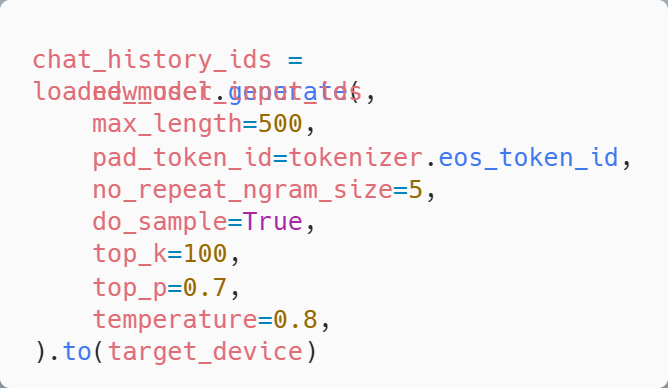
\includegraphics[width=0.8\textwidth]{fundation}}
	\caption{پیکربندی سیستم}
	\label{fig:fundation}
\end{figure}

آزمایش‌های فرعی جهت ارزیابی قسمت‌های مختلف دخیل در فرآیند پروفایل‌سازی کاربر به شرح زیر دسته‌بندی می‌شوند.
\begin{itemize}
\item
بدون ماژول تحلیل معنایی
\item
بدون فیلتر مشارکتی: صرف نظر از محاسبات شباهت و توصیه‌های مستقیم.
\item
ورودی توکن کاهش/افزایش‌یافته: مقایسه کیفیت کار و پیشنهادهای تولیدی سیستم زمانی که بیشینه طول عبارت تولیدی توسط سیستم کاهش یا افزایش باید.
\end{itemize}

در جدول 
\ref{tab:SensitivityAnalysis}
مقایسه تغییر مقادیر معیارهای ارزیابی معرفی‌شده با استفاده از آنالیز حساسیت بر روی قسمت‌های مختلف سیستم آورده شده است.

% جدول مقایسه معیارهای ارزیابی با استفاده از آنالیز حساسیت
\setlength{\extrarowheight}{0pt} % No extra space

\begin{table}[ht]
    \centering
    \caption{مطالعه فرسایشی}
    \label{tab:SensitivityAnalysis}
    \renewcommand{\arraystretch}{1} % Adjusts row height
    \onehalfspacing
    \begin{tabularx}{0.91\textwidth}{|
             >{\centering\arraybackslash}m{3.6cm}|
             >{\centering\arraybackslash}m{0.9cm}|
             >{\centering\arraybackslash}m{0.9cm}|
             >{\centering\arraybackslash}m{0.9cm}|
             >{\centering\arraybackslash}m{0.9cm}|
             >{\centering\arraybackslash}m{1.2cm}|
             >{\centering\arraybackslash}m{0.9cm}|
             >{\centering\arraybackslash}m{0.9cm}|} % Updated column count
        \hline
        \rotatebox{0}{معیارهای ارزیابی} & 
        \rotatebox{90}{Perplexity} &         
        \rotatebox{90}{ \text{\num{Distinct-1}}} & 
        \rotatebox{90}{ \text{\num{Distinct-2}}} & 
        \rotatebox{90}{\text{\num{SuccessRate}}} & 
        \rotatebox{90}{\text{\num{CompletionRate}}} & 
        \rotatebox{90}{UES} & 
        \rotatebox{90}{PDM} \\ % Ensure header matches columns
        \hline
        \rotatebox{0}{سیستم کامل} & 
        \textbf{\num{8.84}} &         
        \text{\num{0.26}} & 
        \text{\num{0.58}} & 
        \textbf{\num{91.97}} & 
        \textbf{\num{93.87}} & 
        \textbf{\num{91.97}} & 
        \textbf{\num{94.29}} \\
        \hline
        \rotatebox{0}{بدون تحلیل معنایی} & 
        \text{\num{9.50}} &         
        \text{\num{0.22}} & 
        \text{\num{0.5}} & 
        \text{\num{88}} & 
        \text{\num{90}} & 
        \text{\num{88}} & 
        \text{\num{91}} \\
        \hline
        \rotatebox{0}{بدون فیلتر مشارکتی} & 
        \text{\num{9.30}} &         
        \text{\num{0.24}} & 
        \text{\num{0.54}} & 
        \text{\num{89}} & 
        \text{\num{91}} & 
        \text{\num{89}} & 
        \text{\num{92.5}} \\
        \hline
        \rotatebox{0}{کاهش طول خروجی مدل} & 
        \text{\num{10.20}} &         
        \text{\num{0.18}} & 
        \text{\num{0.45}} & 
        \text{\num{85}} & 
        \text{\num{88}} & 
        \text{\num{85}} & 
        \text{\num{89}} \\
        \hline
        \rotatebox{0}{بدون پروفایل کاربری} & 
        \text{\num{11.50}} &         
        \textbf{\num{0.15}} & 
        \textbf{\num{0.4}} & 
        \text{\num{80}} & 
        \text{\num{83}} & 
        \text{\num{80}} & 
        \text{\num{85}} \\
        \hline
    \end{tabularx}
\end{table}





\subsection{تاثیر ماژول پروفایل کاربری بر رضایت کاربران}
مشاهدات از آنالیز حساسیت بخش پروفایل سازی کاربربه شرح زیر است.

\subsubsection{ماژول تحلیل معنایی}

همانطور که انتظار می‌رفت، حذف برچسب‌گذاری احساسات باعث کاهش امتیازهای معیارهای ارزیابی مرتبط به پروفایل کاربری شده‌است، زیرا نشانه‌های زمینه‌ای خاص ژانر یا برچسب از بین می‌رود.

معیارهای PRA و PDM زمانی که این مؤلفه حذف می‌شود، دقت و اثربخشی پروفایل را کاهش می‌دهد. 

\subsubsection{ماژول فیلتر مشارکتی}

با حذف ماژول فیلتر مشارکتی مبتنی بر آیتم کاهش متوسط ​​در میزان موفقیت و تکمیل قابل مشاهده است، زیرا توصیه‌های شخصی‌شده حذف می‌شوند.
همچنین معیارهای PRA و PDM نشان‌دهنده کاهش جزئی به دلیل عدم وجود بینش مشترک بین پروفایل کاربر و نتایج تولیدشده توسط مدل است.

\subsubsection{بدون هیچ‌ گونه پروفایل کاربری}

بالاترین گیجی و کمترین UES، که منعکس‌کننده شخصی‌سازی و تعامل ضعیف است. معیارهای PRA و PDM در پایین‌ترین حد خود قرار دارند که نشان‌دهنده حداقل مشارکت در پروفایل کاربری است.

\subsection{تاثیر کاهش طول بیشینه متن تولیدی توسط مدل}

تخریب قابل توجه در معیارهای تمایز و موفقیت به‌دلیل زمینه محدود برای تولید پاسخ، که ناشی از اتکای مدل به داده‌های ورودی گسترده‌تر و تولید متن طولانی‌تر برای حفظ انسجام و ایجاد پاسخ‌های متنوع است. این نشان می‌دهد که کاهش طول ورودی، توانایی مدل را برای استفاده مؤثر از داده‌های پروفایل کاربر و تاریخچه گفتگو، و همچنین ارایه پیشنهاد در متن خروجی که برای تولید پاسخ‌های ظریف و شخصی‌شده حیاتی هستند، محدود می‌کند.


معیارهای PRA و PDM منعکس کننده تأثیر منفی گسترده‌تری بر تصمیمات پروفایل است.

% \subsection{تاثیر استفاده از حق فراموشی در کیفیت خروجی مدل}



\subsection{جمع بندی}
تجزیه و تحلیل حساسیت نشان می‌دهد که چگونه تکنیک‌های پروفایل کاربر به طور مستقیم با برجسته‌کردن تأثیر آنها بر معیارهایی مانند PRA، PDM و UES به عملکرد سیستم کمک می‌کند. 

این تجزیه و تحلیل همچنین زمینه‌های بالقوه برای بهینه‌سازی، مانند پالایش اجزای فیلتر مشارکتی یا تجزیه و تحلیل معنایی را روشن می‌کند و در نتیجه راه را برای تعامل کاربر افزایش‌ یافته و سیستم‌های گفتگوی قوی‌تر در آینده هموار می‌کند. ردیابی امتیازات PRA و PDM بینش بیشتری در مورد اثربخشی روش های پروفایل ارائه می‌دهد. این یافته‌ها بهینه‌سازی بیشتر سیستم گفتگو و بهبود رضایت کاربر را راهنمایی می‌کند.

\section{نتایج نهایی و مقایسه با کارهای موجود}

\subsection{نتایج نهایی}
در این بخش با تاکید بر ایجاد یک سیستم گفتگوی شخصی با استفاده از تکنیک‌های تنظیم سریع و پروفایل کاربری، عملکرد سیستم را از طریق معیارهای مختلفی ارزیابی کردیم. که کیفیت پاسخ های تولید‌شده، تعامل سیستم و رضایت کاربر را ارزیابی شده است. 

روش‌شناسی در اینجا شامل استفاده از سیستم‌های گفتگوی وظیفه‌محور است که با تنظیم سریع بهبود یافته‌اند، جایی که مدل در طول زمان با ترجیحات کاربر سازگار می‌شود. برای ارزیابی عملکرد سیستم، مجموعه‌ای از معیارهای کلیدی را به کار می‌گیریم، از جمله:

نتایج نهایی عملکرد سیستم فوق را در تمامی معیارهای کلیدی به شرح زیر است.

\begin{LTR}
\begin{itemize}

\item
\text{Perplexity} : 8.84
\item
\text{Distinct-1} : 0.26 
\item
\text{Distinct-2} : 0.58
\item
\text{SuccessRate} : 91.97%
\item
\text{CompletionRate} : 93.87%
\item
\text{UES} : 91.97%
\item
\text{PRA}: 76.41%
\item
\text{PDM}: 94.29%

\end{itemize}
\end{LTR}


\subsection{مقایسه با کارهای موجود}

\begin{enumerate}
\item
گیجی: گیجی سیستم فوق مقدار 
 \num{8.84}
 است که کمتر از مدل بیان‌شده در مقاله %
\cite{madotto2021few}

با کیمنه مقدار
 \lr{9.5}
 و همچنین کمتر از مقدار بیان‌شده در مقاله %
\cite{chung2023instructtods}
با مقدار 
\num{36.63}

است، که نشان می‌دهد مدل در مقایسه با مقالات بیان‌شده در پیش‌بینی‌های خود اطمینان بیشتری دارد. این اختلاف می‌تواند به دلیل ماهیت خاص دامنه و بهبودهای انجام شده هنگام تنظیم سریع مدل باشد.

\item
معیار دیستینک-1: امتیاز مدل بیان شده 
 \num{0.26}
 است که با امتیاز گزارش شده در مقاله%
\cite{kasahara2022building}
\num{0.231}
 مطابقت دارد. این نشان می‌دهد که مدل فوق نسبت به تعداد کل تک‌گرم‌ها، یونی‌گرام‌های منحصربه‌فرد بیشتری تولید می‌کند، که نشان‌دهنده تنوع واژگانی بالاتر در سطح یونیگرام است.

\item
معیار دیستینک-2: مقاله 
\cite{kasahara2022building}
در مقایسه با کار مدل بیان شده با امتیاز 
\num{0.58}
 دارای امتیاز کمی بالاتر 
\num{0.595}

است. این نشان می‌دهد که مدل این مقاله نسبت به تعداد کل بای گرام‌ها، بای گرام‌های منحصربه‌فرد بیشتری تولید می‌کند که نشان‌دهنده تنوع واژگانی اندکی بالاتر در سطح بای‌گرام است.

\item
میزان موفقیت: میزان موفقیت در سیستم فوق 
\num{91.79}
 متفاوت از آنچه در InstructTODS ارائه شده است.
مقاله «InstructTODS: مدل‌های زبان بزرگ برای سیستم‌های گفتگوی وظیفه‌محور انتها به انتها»
\cite{chung2023instructtods}
 نرخ موفقیت را به عنوان معیاری از توانایی سیستم گفتگو برای دستیابی به هدف کاربر تعریف می‌کند. بر این اساس محاسبه می‌شود که آیا سیستم وظیفه درخواست‌شده توسط کاربر را با موفقیت انجام می‌دهد یا خیر. این مقاله مقدار نهایی
\num{78.48}
را برای میزان موفقیت خود ارایه داده است.

همچنین در 
\cite{hu2024dialight}
این مقدار به صورت میانگین برابر با 
\num{85.1}
محاسبه می‌شود. 


برای معیارهایی مانند میزان موفقیت، که در آن آثار مختلف از تعاریف متفاوتی استفاده می‌کنند تفاوت در روش‌های محاسبه باید مورد توجه قرار گیرد، زیرا ما از یک تعریف سفارشی بر اساس تکمیل کار استفاده می‌کنیم، در حالی که InstructTOD ممکن است شامل عوامل اضافی باشد اما تعریف نهایی همه در حیطه به انجام ‌رساندن وظیفه محول‌شده به سیستم گفتگو یکسان است.

در ارزیابی فوق میزان موفقیت را بر اساس تعداد کارهایی که با موفقیت توسط سیستم انجام شده است، با توجه به تشخیص قصد و دقت پاسخ محاسبه می‌کنیم.

\end{enumerate}


\subsection{ارزیابی انسانی}
علاوه بر ارزیابی‌های سیستماتیک بیان شده، یک ارزیابی انسان-هوش مصنوعی انجام شده است که در آن ده ارزیابی انسانی با سیستم فوق تعامل داشتند و در مورد جنبه‌های مختلف عملکرد سیستم بازخورد ارائه می‌کردند. در زیر نتایج آماری برای بازخورد انسانی آورده شده است.

نتایج ارزیابی‌های انسانی انجام‌شده به همراه ارسال همان سوالات و پاسخ‌ها به مدل هوش مصنوعی جی‌پی‌تی 
\num{3.5}
جهت انجام ارزیابی هوشمند و مقایسه آن در جدول 
\ref{tab:ComparisonGPT35}
آورده شده است.
\begin{table}[ht]
    \caption{مقایسه نتایج ارزیابی انسان و مدل}
    \label{tab:ComparisonGPT35}
    \centering
    \onehalfspacing
    \begin{tabularx}{\textwidth}{|>{\centering\arraybackslash}X|>{\centering\arraybackslash}X|>{\centering\arraybackslash}X|}
        \hline
        \rotatebox{0}{معیارها} & 
        \rotatebox{0}{ارزیابی انسان} &         
        \rotatebox{0}{ارزیابی هوش مصنوعی}  \\
        \hline
        \rotatebox{0}{Perplexity} & 
        \num{13.49} &         
        \num{13.09} \\
        \hline
        \rotatebox{0}{1Distinct} & 
        \num{0.29} &         
        \num{0.29} \\
        \hline
        \rotatebox{0}{2Distinct} & 
        \num{0.60} &         
        \num{0.60} \\
        \hline
        \rotatebox{0}{Rate Success} & 
        \num{84.42} &         
        \num{85.29}\\
        \hline
        \rotatebox{0}{Rate Completion} & 
        \num{94.19} &         
        \num{93.89}  \\
        \hline
        \rotatebox{0}{UES} & 
        \num{79.57} &         
        \num{85.29}  \\
        \hline
    \end{tabularx}
\end{table}

\begin{itemize}
\item
گیجی: ارزیابی انسان برای گیجی تقریباً با نتایج مدل هوش‌مصنوعی یکسان است.
این نشان می‌دهد که پاسخ‌های این مدل برای انسان‌ها به همان اندازه که برای خود سیستم هوش‌مصنوعی گیج‌کننده است.
\item
دیستنیک ۱و ۲: هر دو معیار بین ارزیابی‌های انسان و هوش‌مصنوعی سازگار هستند، که نشان می‌دهد این مدل پاسخ‌های مشابهی را در تعاملات انسانی ایجاد می‌کند که در ارزیابی‌های هوش‌مصنوعی انجام می‌دهد.
\item
میزان موفقیت: میزان موفقیت در ارزیابی انسانی در مقایسه با نتایج مدل هوش‌مصنوعی کمی کمتر است. این اختلاف را می‌توان به ماهیت ذهنی ارزیابی انسانی نسبت داد، جایی که کاربران ممکن است همیشه در مورد تکمیل کامل یک کار به توافق نرسند.
\item
نرخ تکمیل: میزان تکمیل در هر دو ارزیابی تقریباً یکسان است، با یک تفاوت بسیار کوچک، که نشان می‌دهد سیستم در هر دو ارزیابی پاسخ‌های منسجم و کاملی را ارائه می‌دهد.
\item
 امتیاز تعامل کاربر: در ارزیابی انسانی در مقایسه با هوش‌مصنوعی به طور قابل ‌توجهی کمتر است. این اختلاف ممکن است منعکس‌کننده تفاوت در نحوه درک ارزیابی‌های انسانی از کیفیت تعامل در مقابل ارزیابی داخلی مدل هوش‌مصنوعی باشد.
\end{itemize}

بازخورد انسانی نشان می‌دهد که در حالی که مدل هوش‌مصنوعی در ایجاد پاسخ‌ها عملکرد خوبی دارد، تفاوت‌های ظریفی در نحوه درک انسان از اثربخشی سیستم، به ویژه در مورد تعامل کاربر وجود دارد. این بینش، پیشرفت‌های آینده را در افزایش توانایی سیستم برای تعامل مؤثرتر با کاربران راهنمایی می‌کند.

\subsection{رابط‌کاربری برای ارزیابی انسانی}

برای ارزیابی اثربخشی سیستم گفتگوی وظیفه‌محور و جمع‌آوری بازخورد انسانی، یک رابط کاربری مبتنی بر اپلیکیشن موبایل نیز توسعه داده شد. این رابط کاربری برای تقلید از سناریوهای دنیای واقعی طراحی شده است که در آن کاربران با سیستم‌های توصیه‌ای تعامل دارند و به آنها اجازه می‌دهد:
\begin{itemize}
\item
ثبت ٰژانرهای مورد علاقه: برای همه کابران به‌ویژه برای کاربران نوپا، امکان انتخاب ژانرهای مورد علاقه فراهم است.
\item
 ارسال پرسش‌ها: کاربران عبارت‌های زبان طبیعی را وارد می‌کنند، مانند «آیا می‌توانید یک فیلم اکشن توصیه کنید؟»
\item
 دریافت پاسخ‌ها: سیستم توصیه‌های سریع تنظیم‌شده متناسب با پرس‌و‌جو و نمایه کاربر را ارائه می‌دهد.
\item
 ارائه بازخورد: کاربران می‌توانند با انتخاب یکی از سه گزینه به پاسخ‌ها واکنش نشان دهند: «پسندیدن»، «نپسندیدن» یا «خنثی».
\end{itemize}

هدف اولیه رابط کاربری ارزیابی عملکرد سیستم از نظر موارد زیر بود:
\begin{itemize}
\item
 ارتباط و انسجام: توسط بازخورد کاربر در مورد پاسخ‌های فردی ارزیابی می‌شود.
\item
 تعامل و رضایت: از طریق تعاملات مکرر و ورودی کیفی کاربر اندازه گیری می‌شود.
\item
 تنوع پاسخ: با مشاهده واکنش کاربران به ژانرها یا سبک‌های مختلف پاسخ‌ها ارزیابی می‌شود.
\end{itemize}

این رابط همچنین ثبت تمام تعاملات کاربر را تسهیل کرد و یک مجموعه داده حیاتی را برای ارزیابی انسانی تشکیل داد. این مجموعه داده برای محاسبه معیارهایی مانند امتیاز تعامل کاربر و میزان موفقیت و اعتبارسنجی معیارهای خودکار استفاده شد.

یک نمونه از این رابط کاربری مطابق با شکل%
\ref{fig:MindMeldUi}
 است.

\begin{figure}[ht]
	\centerline{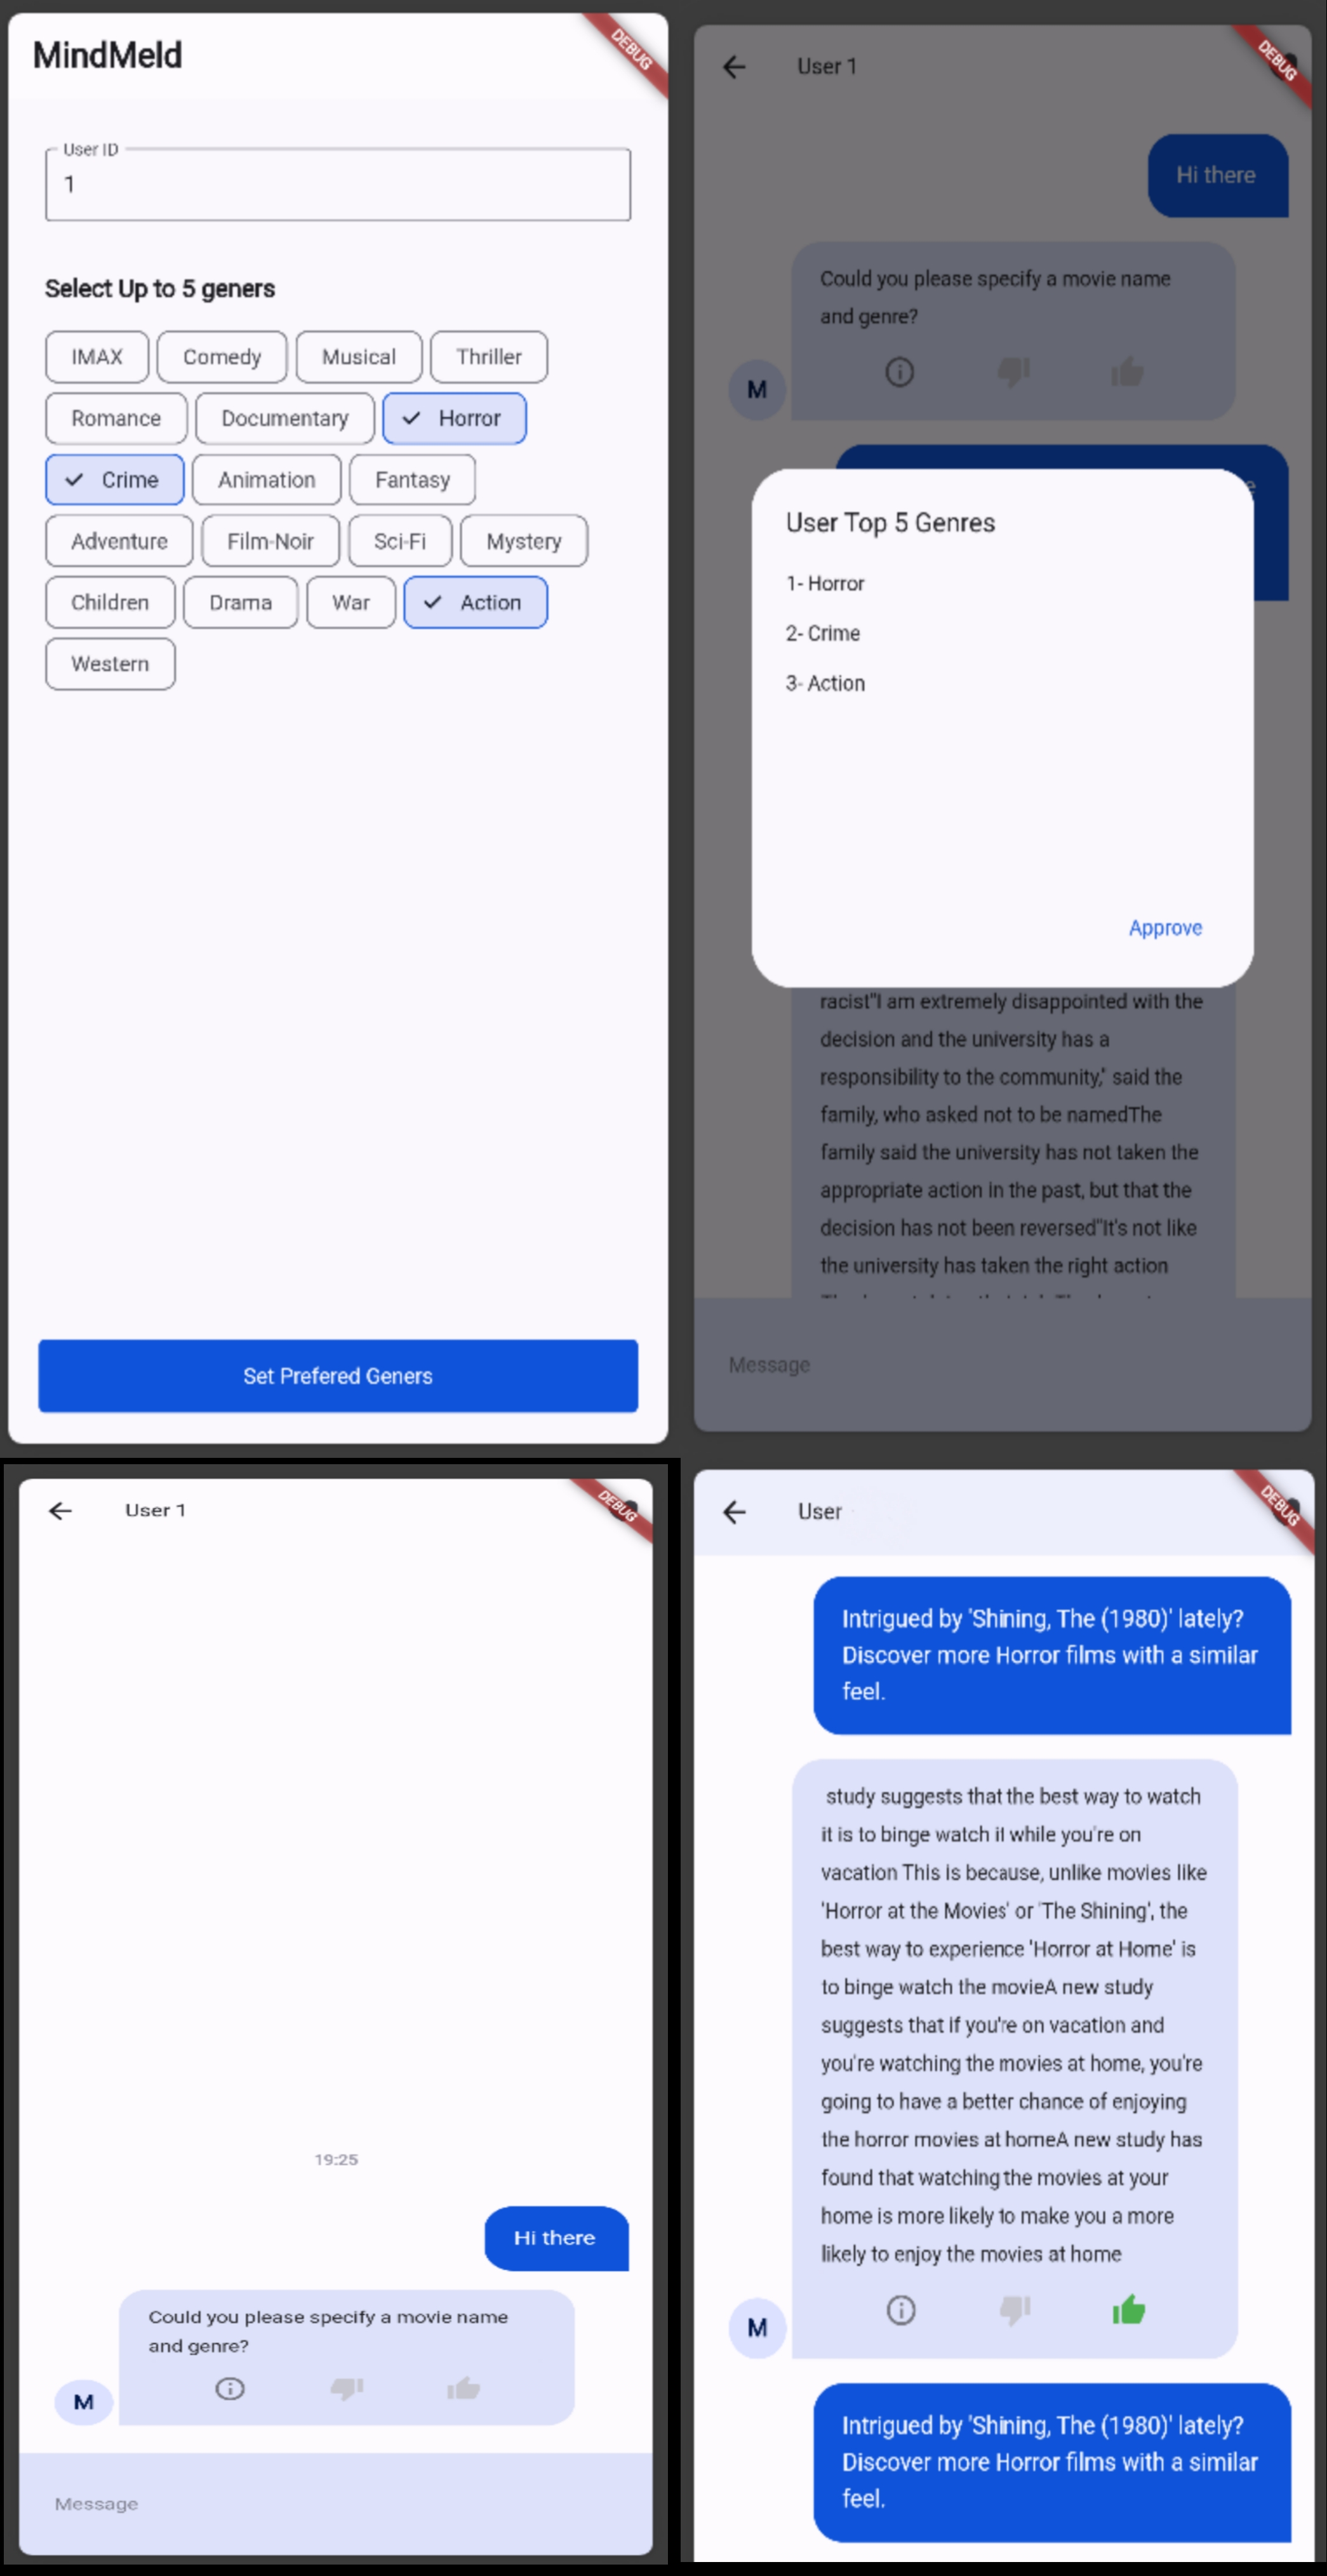
\includegraphics[width=0.5\textwidth]{prototype}}
	\caption{رابط کاربری طراحی‌شده}
	\label{fig:MindMeldUi}
\end{figure}



\section{نتیجه‌گیری}

در این فصل، به طور سیستماتیک مجموعه داده‌های مورد استفاده برای آموزش و ارزیابی مدل را با تمرکز اولیه روی مجموعه داده‌های مووی‌لنز مورد بررسی قرار گرفت. 

این مجموعه داده‌های غنی و متنوعی از تعاملات کاربران ارائه می‌دهد که مبنایی برای کارهای شخصی‌سازی و توصیه‌ها را تشکیل می‌دهد. ویژگی‌های مجموعه داده‌ها، از جمله رتبه‌بندی‌های کاربر، ژانرهای فیلم، و مُهرهای زمانی را که برای ایجاد نمایه‌های دقیق کاربر ضروری بودند، به تفصیل شرح داده شدند. 

مجموعه داده‌های آزمایشی به دقت تنظیم شدند تا عملکرد مدل را تحت سناریوهای واقعی ارزیابی کنند و از مقایسه منصفانه و قابل اعتماد نتایج اطمینان حاصل کنند. علاوه بر این، این فصل در مورد پیکربندی ابرپارامتر که برای افزایش کارایی مدل، از جمله نرخ یادگیری، اندازه دسته و نرخ ترک تحصیل، به خوبی تنظیم شده بودند، توضیح داده‌شد.

نتایج با استفاده از معیارهایی مانند گیجی، تمایز، میزان موفقیت، میزان تکمیل و امتیاز تعامل کاربر و همچنین معیارهای مرتبط به طور مستقیم با پروفایل کاربری مانند دقت توصیه شخصی و تطابق تنوع نمایه ارزیابی شدند. 

این معیارها نقاط قوت و محدودیت‌های مدل را برجسته می‌کنند و نمای شفافی از عملکرد آن در ابعاد مختلف ارائه می‌دهند. تجزیه و تحلیل حساسیت بیشتر استحکام مدل را در برابر تغییرات در پارامترهای کلیدی نشان داد و بر سازگاری و قابلیت اطمینان آن در محیط‌های پویا تأکید کرد. 

این فصل چارچوب آزمایش و ارزیابی دقیق را در بر می‌گیرد که از نتیجه‌گیری‌ها و بینش‌های گسترده‌تر ارائه‌شده در این تحقیق پشتیبانی می‌کند.

سیستم فوق در بسیاری از زمینه‌ها خوب عمل می‌کند، اما فضایی برای بهبود، به ویژه در تعامل با کاربر، همانطور که توسط ارزیابی انسان-هوش‌مصنوعی برجسته شده‌است، نشان می‌دهد.



